% --------------------------------------------------------------
% This is all preamble stuff that you don't have to worry about.
% Head down to where it says "Start here"
% --------------------------------------------------------------
 
\documentclass[12pt]{article}
 
\usepackage[margin=1in]{geometry} 
\usepackage{amsmath,amsthm,amssymb,scrextend}
\usepackage{fancyhdr}
\usepackage{enumitem}
\usepackage{amsmath}
\usepackage{amssymb}
\usepackage{textcomp}
\usepackage{fancybox}
\usepackage{tikz}
\pagestyle{fancy}
\usepackage[makeroom]{cancel}
\usepackage{graphicx}
\usepackage{caption}
\usepackage{mwe}

\newcommand{\N}{\mathbb{N}}
\newcommand{\Z}{\mathbb{Z}}
\newcommand{\I}{\mathbb{I}}
\newcommand{\R}{\mathbb{R}}
\newcommand{\Q}{\mathbb{Q}}
\renewcommand{\qed}{\hfill$\blacksquare$}
\let\newproof\proof
\renewenvironment{proof}{\begin{addmargin}[1em]{0em}\begin{newproof}}{\end{newproof}\end{addmargin}\qed}
% \newcommand{\expl}[1]{\text{\hfill[#1]}$}
 
\newenvironment{theorem}[2][Theorem]{\begin{trivlist}
\item[\hskip \labelsep {\bfseries #1}\hskip \labelsep {\bfseries #2.}]}{\end{trivlist}}
\newenvironment{lemma}[2][Lemma]{\begin{trivlist}
\item[\hskip \labelsep {\bfseries #1}\hskip \labelsep {\bfseries #2.}]}{\end{trivlist}}
\newenvironment{problem}[2][Problem]{\begin{trivlist}
\item[\hskip \labelsep {\bfseries #1}\hskip \labelsep {\bfseries #2.}]}{\end{trivlist}}
\newenvironment{exercise}[2][Exercise]{\begin{trivlist}
\item[\hskip \labelsep {\bfseries #1}\hskip \labelsep {\bfseries #2.}]}{\end{trivlist}}
\newenvironment{reflection}[2][Reflection]{\begin{trivlist}
\item[\hskip \labelsep {\bfseries #1}\hskip \labelsep {\bfseries #2.}]}{\end{trivlist}}
\newenvironment{proposition}[2][Proposition]{\begin{trivlist}
\item[\hskip \labelsep {\bfseries #1}\hskip \labelsep {\bfseries #2.}]}{\end{trivlist}}
\newenvironment{corollary}[2][Corollary]{\begin{trivlist}
\item[\hskip \labelsep {\bfseries #1}\hskip \labelsep {\bfseries #2.}]}{\end{trivlist}}
 
\begin{document}
 
% --------------------------------------------------------------
%                         Start here
% --------------------------------------------------------------

\lhead{Math 632}
\chead{Homework 2}
\rhead{Meenmo Kang}

\noindent
\textbf{Question 1}\\
Consider a discrete time Markov chain with transition probabilities $p(i, j)$, with state space
$\{1, 2, . . . , 10\}$, and assume $X_0 = 3$. Express
$$P(X_6 = 7, X_5 = 3\;|\;X_4 = 1, X_9 = 3)$$
in terms of the (if necessary multi-step) transition probabilities.\\

\vspace{1.5\baselineskip}
\noindent
$$P(X_6 = 7, X_5 = 3\;|\;X_4 = 1, X_9 = 3) 
= \frac{P(X_6 = 7, X_5 = 3, X_4 = 1, X_9 = 3)}{P(X_4 = 1, X_9 = 3)}$$
$$
= \frac{P(X_9 = 3\;|\;X_6=7,X_5=3,X_4=1)\cdot P(X_6=7\;|\;X_5=3,X_4=1)\cdot P(X_5=3\;|\;X_4=1)\cdot P(X_4=1)}{P(X_9=3\;|\;X_4=1)\codt P(X_4=1)}$$

$$
= \frac{P(X_9 = 3\;|\;X_6=7)\cdot P(X_6=7\;|\;X_5=3)\cdot P(X_5=3\;|\;X_4=1)\cdot \cancel{P(X_4=1)}}{P(X_9=3\;|\;X_4=1)\cdot \cancel{P(X_4=1)}}$$



$$
= \frac{P(X_9 = 3\;|\;X_6=7)\cdot P(X_6=7\;|\;X_5=3)\cdot P(X_5=3\;|\;X_4=1)}{P(X_9=3\;|\;X_4=1)}$$

$$
=\frac{p^3(7,3)\cdot p^1(3,7)\cdot p^1(1,3)}{p^5(1,3)}
$$



\newpage
\noindent
\textbf{Question 2}\\
Consider a discrete time Markov chain with transition probabilities $p(i, j)$, with state space
$\{1, 2, . . . , 10\}.$ Assume, moreover, that $T$ is a stopping time with the properties $P_1(T<\infty) = 1$ and $P_1(X_T=3) = 1.$ Express
$$P_1(X_{T+6} = 7, X_{T+5} = 3\;|\;X_{T+4} = 1, X_{T+9} = 3)$$
in terms of the (if necessary multi-step) transition probabilities.\\

\vspace{1.5\baselineskip}
\noindent
We can expand the given conditional probability as below.
$$
P_1(X_{T+6} = 7, X_{T+5} = 3\;|\;X_{T+4} = 1, X_{T+9}=3) = 
\frac{P_1(X_{T+6} = 7, X_{T+5} = 3, X_{T+4} = 1, X_{T+9}=3)}{P_1(X_{T+4} = 1, X_{T+9}=3)} 
$$
\noindent
Since the stopping time $T$ for $P_1$ is finite and $P_1(X_T =3) = 1$, it can be transformed as follows preserving the existing distribution by the strong Markov property.

$$
\frac{P_3(X_{4} = 1, X_{5} = 3, X_{6} = 7, X_{9}=3)}{P_3(X_9 = 3, X_4=1)} 
$$
$$
= \frac{P_3(X_9=3\;|\;X_6=7, X_5=3, X_4=1)\cdot P_3(X_6=7\;|\; X_5=3, X_4=1)\cdot P_3(X_5=3\;|\;X_4=1)\cdot P_3(X_4=1)}{P_3(X_9=3\;|\;X_4=1)\cdot P_3(X_4=1)}
$$
 
$$
= \frac{P(X_9=3\;|\;X_6=7)\cdot P(X_6=7\;|\; X_5=3)\cdot P(X_5=3\;|\;X_4=1)\cdot \cancel{P(X_4=1)}}{P(X_9=3\;|\;X_4=1)\cdot \cancel{P(X_4=1)}}
$$

$$
= \frac{p^3(7,3)\cdot p^1(3,7)\cdot p^1(1,3)}{p^5(1,3)}
$$
\noindent
We obtain the same transition probability as Question 1.

\newpage
\noindent
\textbf{Question 3}\\
Consider the discrete time Markov chain with state space $\{1, 2, 3, 4, 5\}$ and transition matrix
$$P = 
\begin{bmatrix}
    0&0&1&0&0\\
    0.3&0.2&0.1&0.4&0\\
    0&1&0&0&0\\
    0&0&0&0.3&0.7\\
    0&0&0&0.2&0.8\\
\end{bmatrix}
$$

\begin{enumerate}[label=(\alph*)]
    \item Draw the transition graph. Identify the transient and the recurrent states.\\

        \begin{minipage}[t]{0.4\textwidth}
          \centering\raisebox{\dimexpr \topskip-\height}{%
          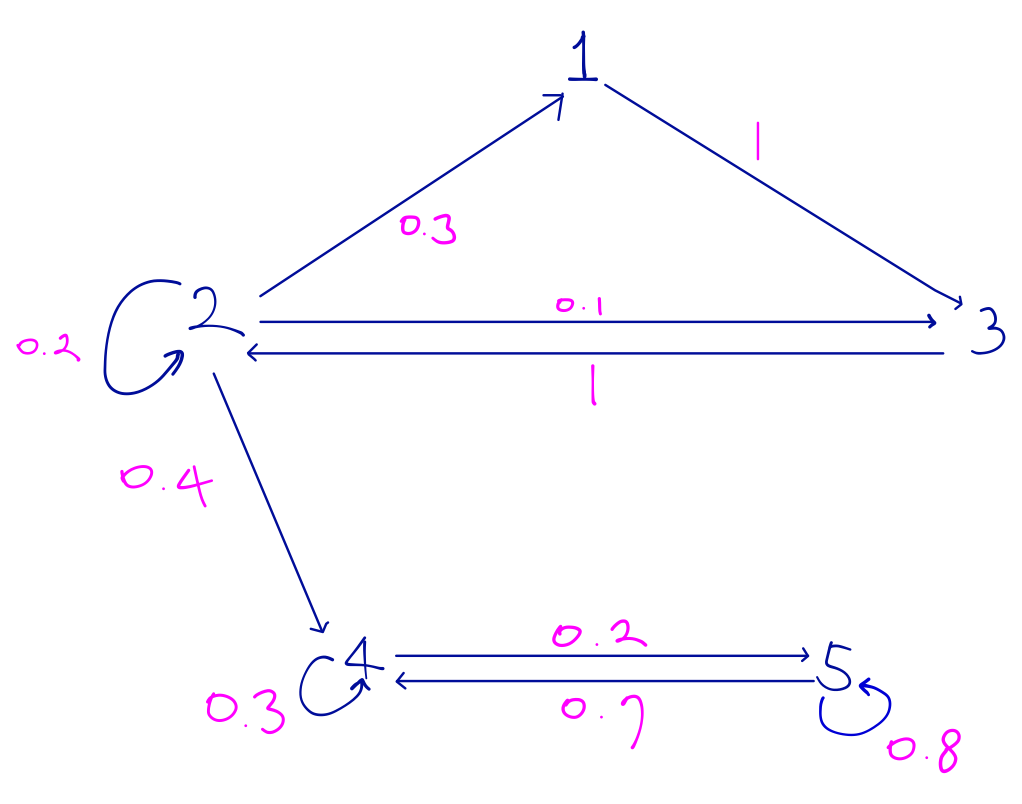
\includegraphics[width=\textwidth]{hw2_capture.png}}
        
        
        \end{minipage}\hfill
        \begin{minipage}[t]{0.65\textwidth}
          \vspace{3\baselineskip}
          \begin{itemize}
          
                \item Transient: $\{1,2,3\}$
                \item Recurrent: $\{4,5\}$
          \end{itemize}
        \end{minipage}



    \item Let $R_2 = max\{n \ge 0: X_n =2\}.$ Prove that $P_2(R_2<\infty) = 1.$
    
        \begin{itemize}
            \item Since $\{4,5\}$ is recurrent, it has to encounter 4 at some point.
            \item Then there is no probability to go back to 2.
            \item Hence it is not possible to stop at 2 infinitely many times\\
            i.e. $R_2$, the last stop at the state 2, is finite.
            \item Thus $P_2(R_2 < \infty) = 1$
        \end{itemize}
    \item Is $R_2$ a stopping time? Why?
        \begin{itemize}
            \item By the definition of stopping time, stopping at time $n$ depends only on the past and present states, or $X_0,...,X_n$.
            \item However, it is impossible to expect when $R_2$ is stopped without consideration of its future status.\\
            e.g.) In case where it goes to 4 and never come back to 2.
            \item Thus $R_2$ is not a stopping time.
        \end{itemize}
    \item Calculate $P_3(X_{R_2+1} = 4\;|\;X_{R_2} = 2, R_2 = 8)$
        \begin{itemize}
            \item Since $8th$ state is the last stop at the state 2, the next state must be 4 where is the recurrent state.
            \item Thus $P_3(X_{R_2+1} = 4\;|\;X_{R_2} = 2, R_2 = 8) = 1$
        \end{itemize}
\end{enumerate}

\vspace{1.5\baselineskip}
\noindent


\newpage
\noindent
\textbf{Question 4}\\
Consider a Markov chain with state space $S = \{1, 2\}$, with transition matrix
$$
P=\begin{bmatrix}
0.2&0.8\\
0.6&0.4
\end{bmatrix}
$$
Decide which of the following is a stopping time:
\begin{enumerate}[label=(\alph*)]
    \item $T_1 = min\{n\ge 6: X_n = 2\}$: Yes
        \begin{itemize}
            \item This is a stopping time since $T_1$ can only be determined by looking at the current state.
        \end{itemize}
    \item $T_2 = min\{n\ge 1: X_{n+1} = 2\}$: No
        \begin{itemize}
        \item Since we need to know the future state $X_{n+1}$ to expect $T_2$, it is not a stopping time.
        \end{itemize}
    \item $T_3 = min\{n\ge 2: X_{n-1} = 2\}$: Yes
        \begin{itemize}
            \item This is a stopping time since it requires to know just the past state for $T_3$.
        \end{itemize}
    \item $T_4 = min\{n\ge T_1: X_{n-1} = 2\}$: Yes
        \begin{itemize}
            \item Since the given $T_1$ considers the current state and the given condition of $T_4$ considers the previous state, not future, it is said to be a stopping time.
        \end{itemize}
    \item $T_5 = min\{n\ge 10: X_n = X_{n-1}\}$: Yes
        \begin{itemize}
            \item This is a stopping time since it requires to know just the previous state for $T_5$.
        \end{itemize}
    \item $T_6 = min\{n\ge 1: X_n = X_5\}$: No
        \begin{itemize}
            \item Similar to (b), we need to know the future state $X_5$, when the current state is $1\le n \le 5$. Hence it is not a stopping time.
        \end{itemize}
    \item $T_7 = 10$: Yes
        \begin{itemize}
            \item $T_7$ is given as 10. We know when and what occurs. Hence $T_7$ is a stopping time.
        \end{itemize}
\end{enumerate}

\vspace{1.5\baselineskip}
\noindent


\newpage
\noindent
\textbf{Question 5}\\
Consider the following transition matrices. Identify the transient and
recurrent states, and the irreducible closed sets in the Markov chains. (No need to give reasons here, but draw the transition
graphs.)
$$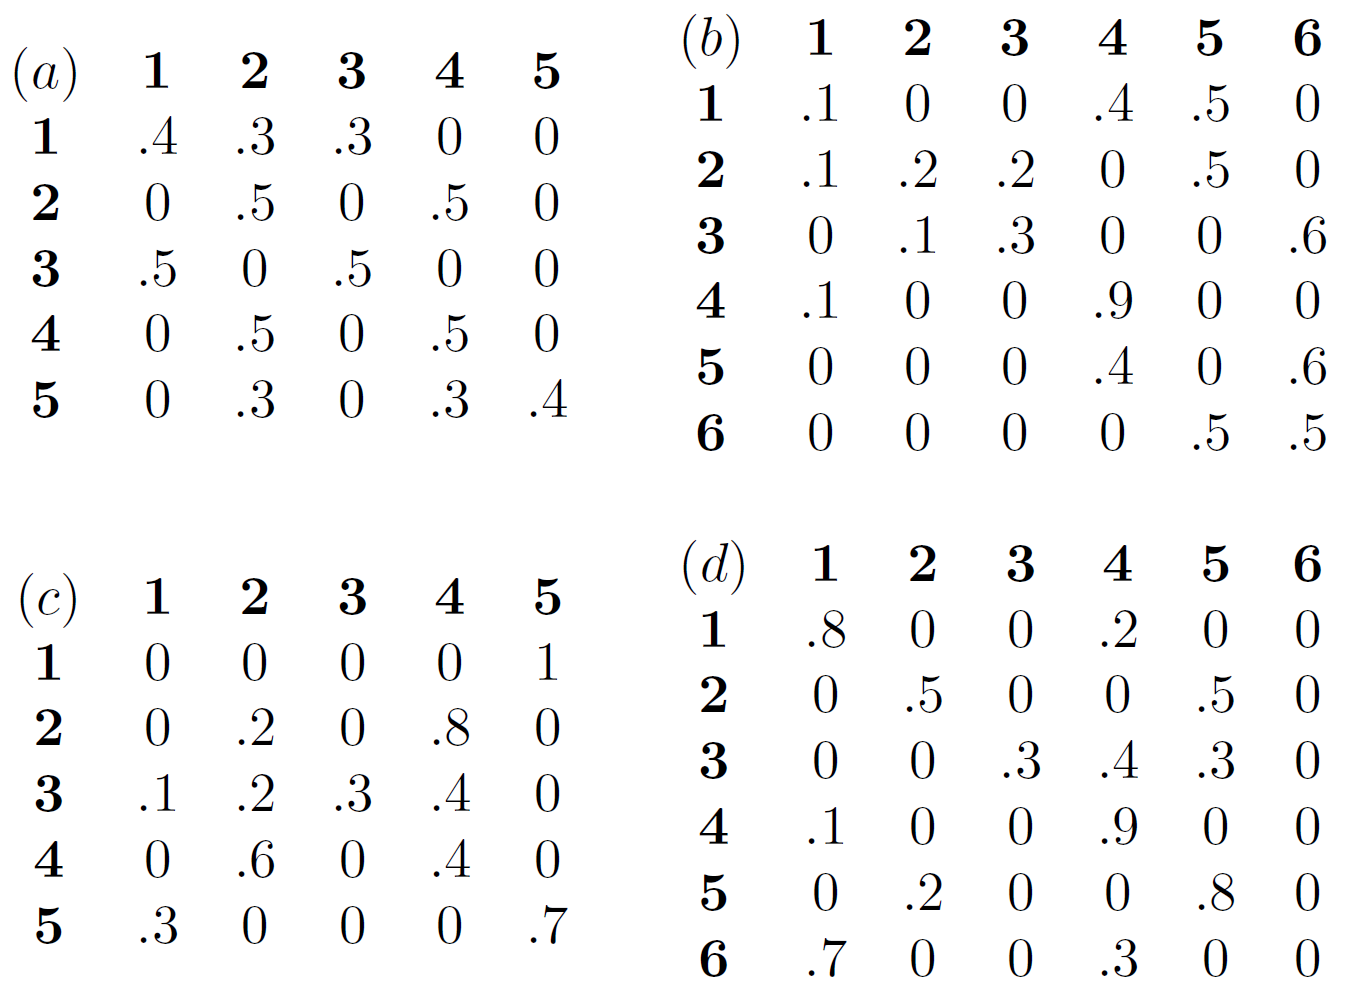
\includegraphics[height=8cm, width=9cm]{hw2_ex8.png}$$

\begin{enumerate}[label=(\alph*)]
\item
        \begin{minipage}[t]{0.4\textwidth}
          \centering\raisebox{\dimexpr \topskip-\height}{%
          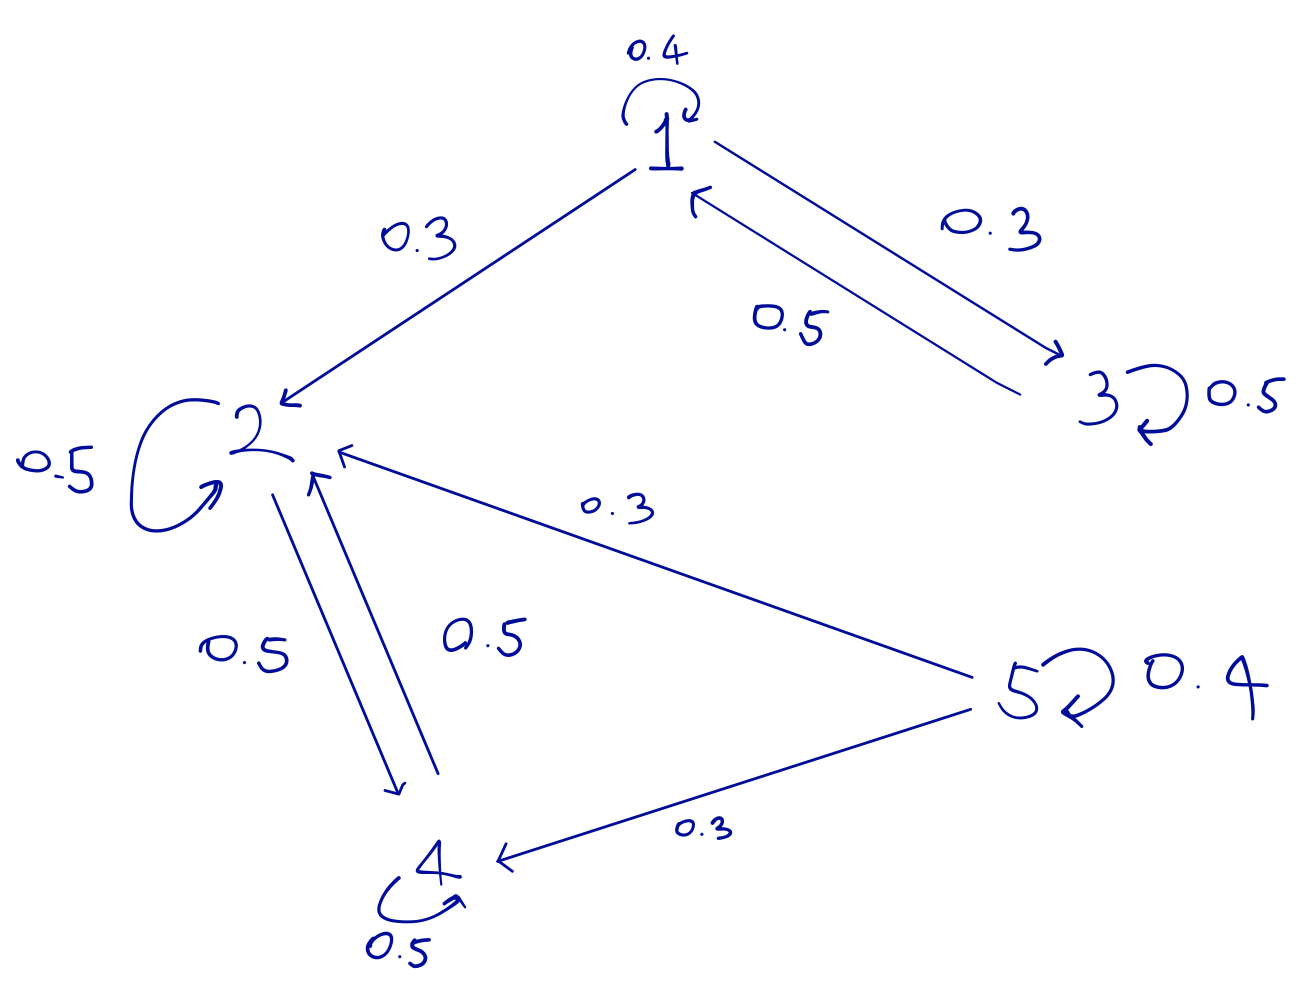
\includegraphics[width=\textwidth]{hw2_8a.png}}
        
        
        \end{minipage}\hfill
        \begin{minipage}[t]{0.65\textwidth}
          \vspace{3\baselineskip}
          \begin{itemize}
                \item Transient Set: $\{1\},\{3\}, \{5\}$
                \item Irreducible Closed Set: $\{2,4\}$
          \end{itemize}
        \end{minipage}


\item
        \begin{minipage}[t]{0.4\textwidth}
          \centering\raisebox{\dimexpr \topskip-\height}{%
          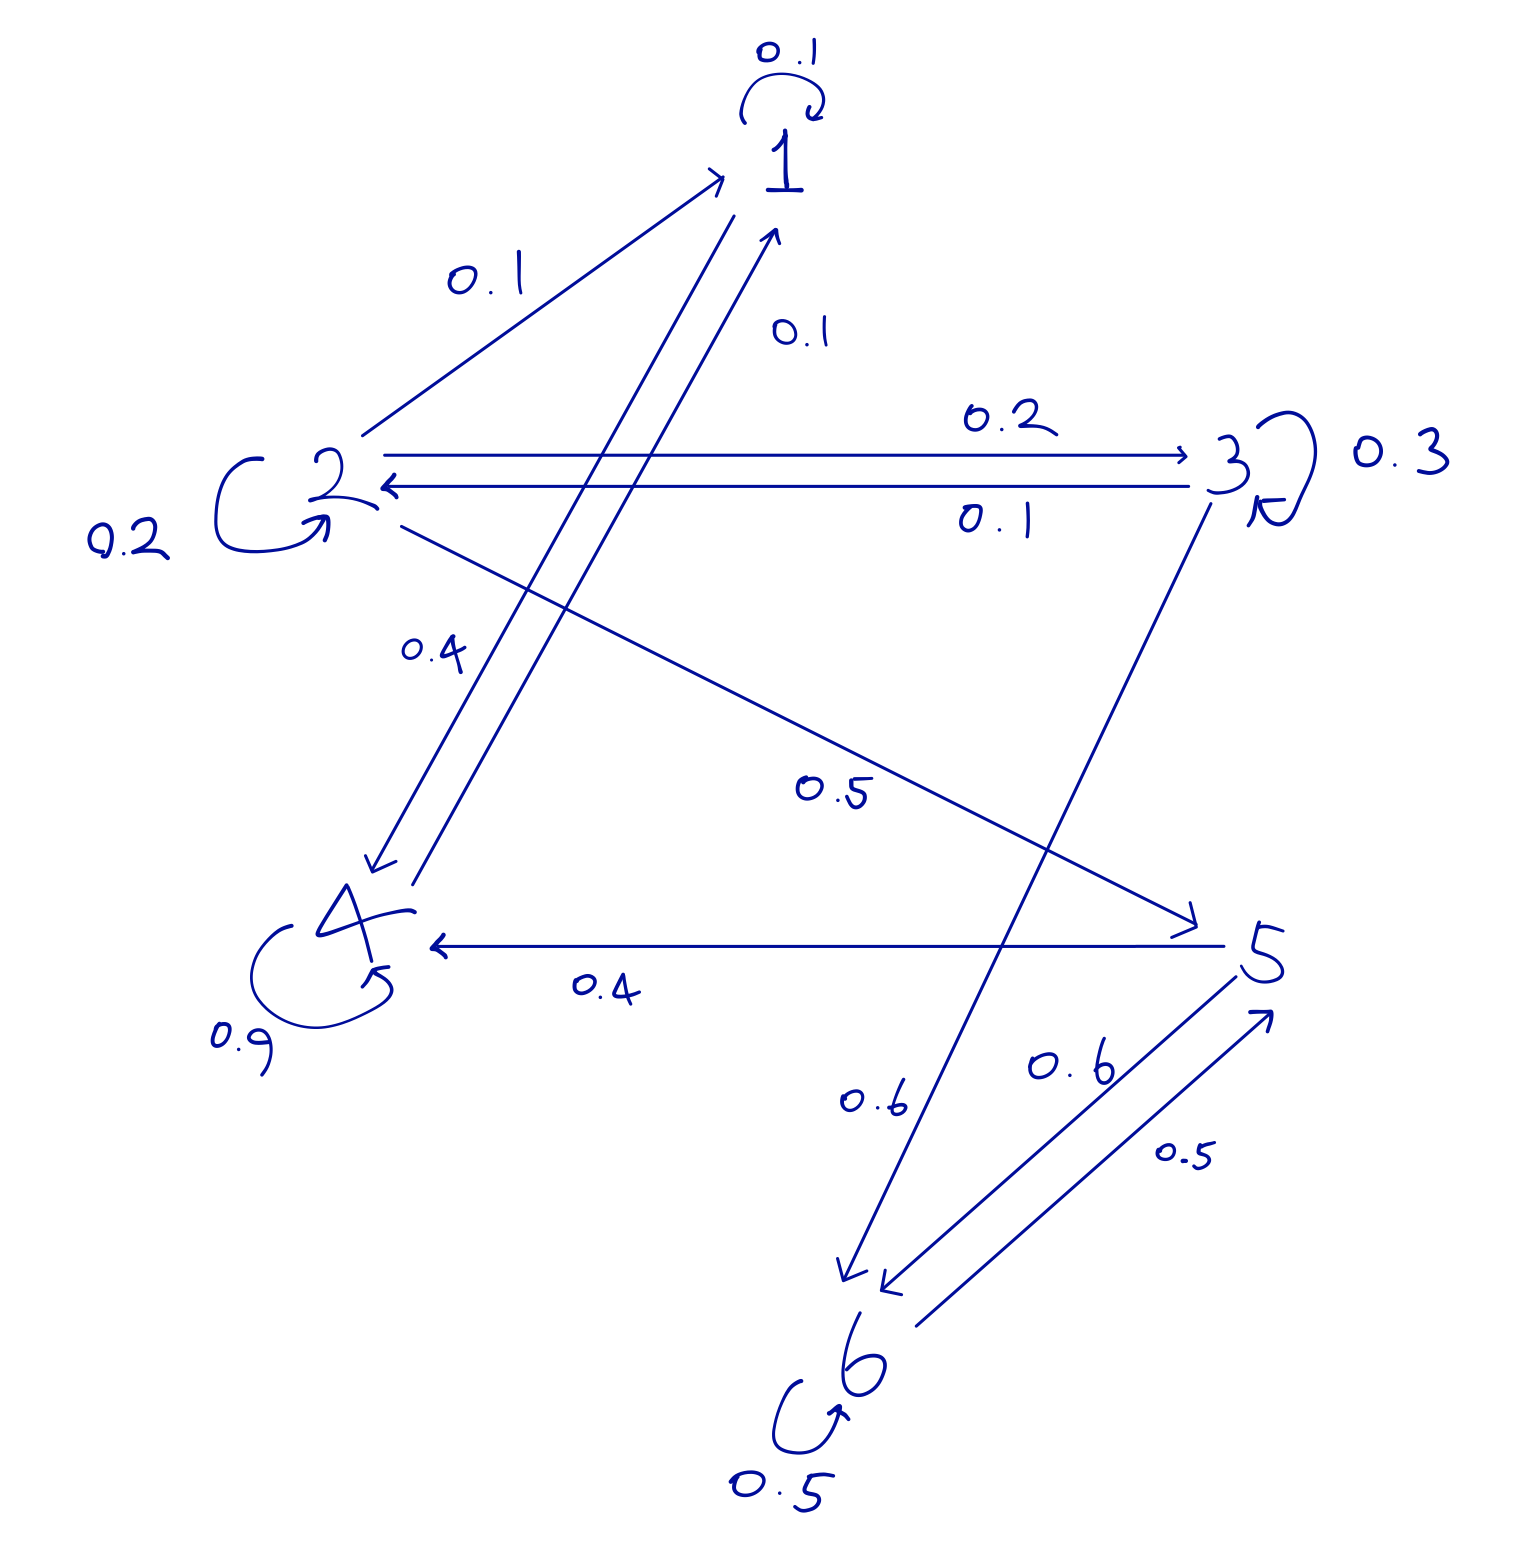
\includegraphics[width=\textwidth]{hw2_8b.png}}
        
        
        \end{minipage}\hfill
        \begin{minipage}[t]{0.65\textwidth}
          \vspace{3\baselineskip}
          \begin{itemize}
                \item Transient Sets: $\{2\}, \{3\}$
                \item Irreducible Closed Sets: $\{1,4,5,6\}$          \end{itemize}
        \end{minipage}
        

\item
        \begin{minipage}[t]{0.4\textwidth}
          \centering\raisebox{\dimexpr \topskip-\height}{%
          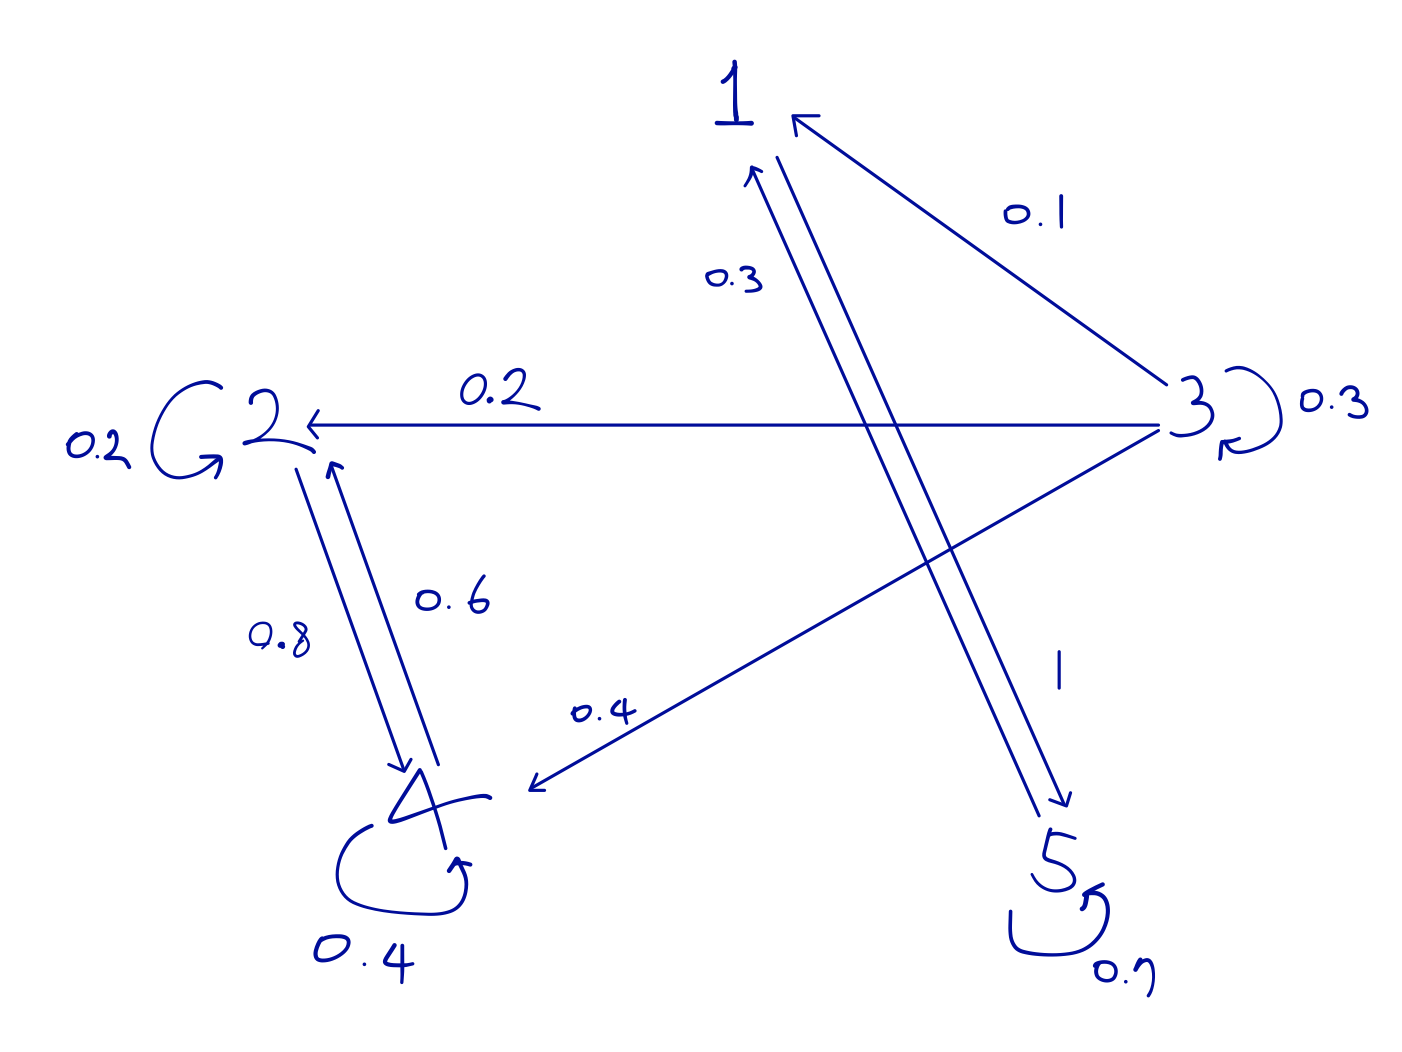
\includegraphics[width=\textwidth]{hw2_8c.png}}
        
        
        \end{minipage}\hfill
        \begin{minipage}[t]{0.65\textwidth}
          \vspace{3\baselineskip}
          \begin{itemize}
                \item Transient Sets: $\{3\}$
                \item Irreducible Closed Sets: $\{1,5\}, \{2,4\}$       
          \end{itemize}
        \end{minipage}
        

\item
        \begin{minipage}[t]{0.4\textwidth}
          \centering\raisebox{\dimexpr \topskip-\height}{%
          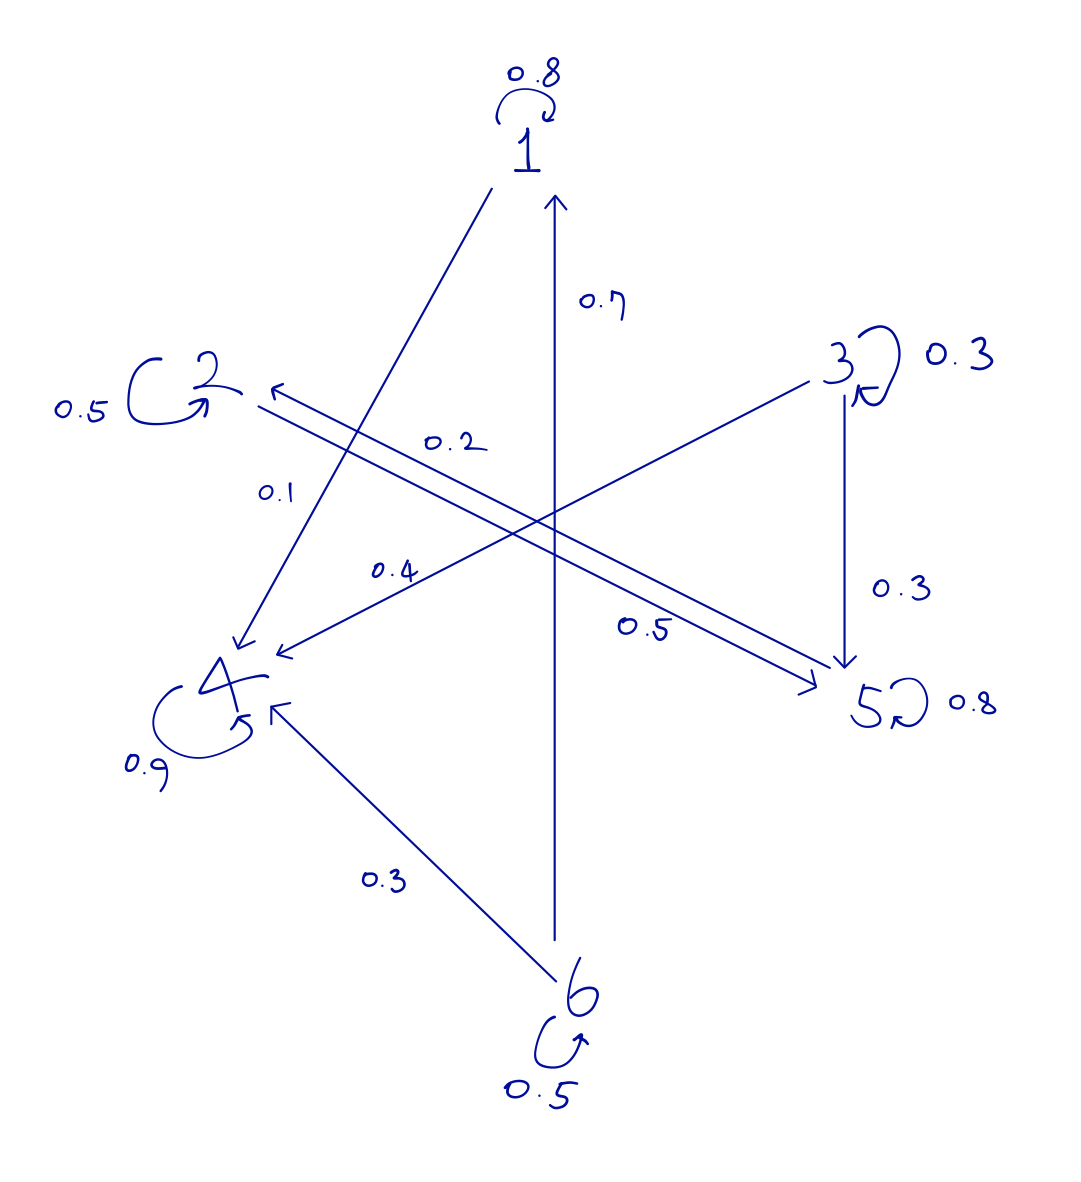
\includegraphics[width=\textwidth]{hw2_8e.png}}
        
        
        \end{minipage}\hfill
        \begin{minipage}[t]{0.65\textwidth}
          \vspace{3\baselineskip}
          \begin{itemize}
                \item Transient Sets: $\{3\}, \{6\}$
                \item Irreducible Closed Sets: $\{2,5\}, \{1,4\}$          
          \end{itemize}
        \end{minipage}
\end{enumerate}


\vspace{1.5\baselineskip}
\noindent


\newpage
\noindent
\textbf{Question 6}\\
Consider a discrete time Markov chain with state space $\mathbb{Z} = \{. . . ,−2,−1, 0, 1, 2, . . . \}$ and one
step transition probabilities given by
$$p(i,i+1) = p \qquad \text{for all } i\in \mathbb{Z}$$
$$p(i,i-1) = q \qquad \text{for all } i\in \mathbb{Z}$$
and zero otherwise, with $p,q\ge 0$ and $p + q = 1$. (This is simple random walk.)

\begin{enumerate}[label=(\alph*)]
    \item Assume that $p = 0$. Find all the closed sets.\\
    
        Since $p=0\Leftrightarrow q=1$, it goes to only backwards. Hence the closed set is 
        $$A_j = \{i \le j\;|\;\forall i \in \mathbb{Z} \} \text{ for all integer $j$}.$$
    \item Assume that $p = 0$. Find all the irreducible sets.\\
    
        We know that $i\to j$ if and only if $j\le i$. Hence, no irreducible set can contain two states $i<j$, because we have $i\to j$. It follows that irreducible sets have at most one state. Besides, all sets of the form$\{i\}$ for some $i\in \mathbb{Z}$ are irreducible, because we always have $i\to i$. These sets are therefore all the irreducible sets of the chain for $p=0$.
    

    \item Now assume that $p, q > 0$. Prove this statement: either all the states are recurrent or all the states are transient.
        \begin{itemize}
            \item Suppose $\exists\; i \in \mathbb{Z}$. Then obviously $i$ communicates with $j$ such that $j = i + 1$ when $p(i,j) = p$. 
            \item In case of $p(j,i) = q$, $j$ communicates with $i$ backwards.
            \item In other words, the state $i$ is recurrent. 
            \item By Lemma 1.9 on Durrett, there states that if $x$ is recurrent, and $x \rightarrow y$, the $y$ is recurrent. 
            \item Thus $\forall \text{ state $i$} \in \mathbb{Z}$ are recurrent.
        \end{itemize}        
        
\end{enumerate}


\vspace{1.5\baselineskip}
\noindent

\newpage
\noindent
\textbf{Question 7}\\
Let $\{X_n\}_{n\ge 0}$ be a Markov Chain with transition probability $\{p(x,y)\}_{x,y\in \mathbb{S}}$ with some countable state space $\mathbb{S}$. That is , the process satisfies

\begin{align}
P(X_{n+1} = y\;|\; X_n = x_n,...,X_0=x_0) = p(x_n,y) 
\end{align}
for all states $x_0, . . . , x_n, y$ such that the conditioning event has positive probability.
\begin{enumerate}[label=(\alph*)]
    \item Using (1) (and general properties of probability and conditional probability), show that
    for any $0 < k\le n,$
    
    \begin{align}
        P(X_{n+1} = y\;|\;X_n = x_n,...,X_k =x_k) = p(x_n,y)
    \end{align}
whenever the conditioning event has positive probability.\\

$$P(X_{n+1} = y\;|\;X_n = x_n,...,X_k =x_k)
=\frac{P(X_{n+1} = y,X_n = x_n,...,X_k =x_k)}{P(X_n = x_n,...,X_k =x_k)}$$
$$
= \frac{P(X_{n+1}=y|X_n=x_n)\cdot P(X_{n}=x_n|X_{n-1}=x_{n-1}) \ldots P(X_{k+1}=x_{k+1}|X_k = x_k)\cdot P(X_k=x_k)}
{P(X_n=x_n|X_{n-1}=x_{n-1})\ldots P(X_{k+1}=x_{k+1}|X_k = x_k)\cdot P(X_k=x_k)}
$$

$$
= \frac{P(X_{n+1}=y|X_n=x_n)\cancel{P(X_{n}=x_n|X_{n-1}=x_{n-1})} \ldots \cancel{P(X_{k+1}=x_{k+1}|X_k = x_k)} \cancel{P(X_k=x_k)}}
{\cancel{P(X_n=x_n|X_{n-1}=x_{n-1})}\ldots \cancel{P(X_{k+1}=x_{k+1}|X_k = x_k)}\cdot \cancel{P(X_k=x_k)}}
$$
$$
=P(X_{n+1}=y|X_n=x_n)
$$
\newpage
\item Using (2), show that
$$
P(X_{n-1} = x, X_{n+1} = z\;|\;X_n = y) = P(X_{n-1} = x\;|\;X_n = y) \cdot P(X_{n+1} = z\;|\;X_n = y)
$$
for all states $x, y, z$ such that $P(X_n = y) > 0$. This is a special case of the statement
that for a Markov chain, \textit{given the present, the past and the future are independent}.\\

$$
P(X_{n-1} = x, X_{n+1} = z\;|\;X_n = y) = \frac{P(X_{n-1}=x,X_n=y,X_{n+1}=z)}{P(X_n=y)}
$$

$$
=\frac{P(X_{n+1}=z|X_n=y)\cdot P(X_{n}=y|X_{n-1}=x)\cdot P(X_{n-1}=x)}{P(X_n=y)}
$$

$$
=
\frac{P(X_{n+1}=z,X_n=y)}{P(X_n=y)}\cdot 
\frac{P(X_{n}=y,X_{n-1}=x)}{P(X_{n-1}=x)}\cdot 
P(X_{n-1}=x)\cdot
\frac{1}{P(X_n=y)}
$$

$$
=
\frac{P(X_{n+1}=z,X_n=y)}{P(X_n=y)}\cdot 
\frac{P(X_{n}=y,X_{n-1}=x)}{\cancel{P(X_{n-1}=x)}}\cdot 
\cancel{P(X_{n-1}=x)}\cdot
\frac{1}{P(X_n=y)}
$$

$$
=
\frac{P(X_{n+1}=z,X_n=y)}{P(X_n=y)}\cdot 
\frac{P(X_{n}=y,X_{n-1}=x)}{P(X_n=y)}
=
P(X_{n+1=x}|X_n=y) \cdot P(X_{n-1}=x|X_n=y)
$$
\end{enumerate}


\end{document}